\documentclass{article}

\usepackage{amsmath}
\usepackage{amssymb}
\usepackage{algorithm}
\usepackage[noend]{algpseudocode}		% for algorithms in pseudo code. Usage: \begin{algorithmic}
\MakeRobust{\Call}
\usepackage{tikz}	% for diagrams
\usetikzlibrary{positioning}
\usetikzlibrary{quotes}

\setlength{\parskip}{\smallskipamount}

\title{Analysis of Algorithms \\
\medskip
\large Homework 4}
\author{Abraham Murciano}

\begin{document}

\maketitle

\section{Dijkstra's Algorithm with negative weights}

\subsection*{Part A}

Figure \ref{q1a} shows a graph with negative weights such that if we apply Dijkstra's algorithm to find the shortest path between vertices \(S\) and \(D\), it will return the wrong path.

\begin{figure}[h]
	\centering
	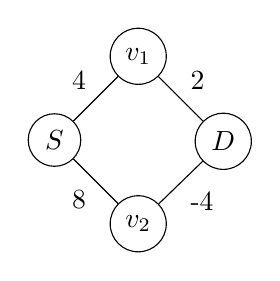
\begin{tikzpicture}
		[vertex/.style={circle, draw=black, node distance=0.8cm}]
		\node[vertex] (S) {\(S\)};
		\node[vertex, above right=of S] (v1) {\(v_1\)};
		\node[vertex, below right=of S] (v2) {\(v_2\)};
		\node[vertex, below right=of v1] (D) {\(D\)};
		\draw (S) to["4"] (v1);
		\draw (S) to["8" below left] (v2);
		\draw (v1) to["2"] (D);
		\draw (v2) to["-4" below right] (D);
	\end{tikzpicture}
	\caption{Graph for which Dijkstra doesn't work}
	\label{q1a}
\end{figure}

Starting off, we assign the unvisited vertices \(v_1\) and \(v_2\) with the distances 4 and 8 respectively, marking \(S\) as visited. Then we take the unvisited vertex with the smallest distance, \(v_1\), and check its neighbours, namely \(D\). We assign it the distance 6 and mark \(v_1\) as visited. Now that our destination vertex is the unvisited vertex with the shortest distance, the algorithm would claim that it has finished, with the shortest path going through \(v_1\) with a distance of 6.

However, in reality the shortest path goes through \(v_2\) and has a total distance of \(8 - 4 = 4\). This path was not considered by the algorithm because the path to the intermediate vertex \(v_2\) has a larger distance than the path it found first.

\subsection*{Part B}

If we take the example graph in figure \ref{q1a} and modify it so that the edges are directed (away from \(S\) or towards \(D\)), then that would form a directed acyclic graph for which Dijkstra's algorithm would not work for a similar reason to that of part A.

\section{Floyd-Warshall with Negative Cycles}

We are to add pseudocode to the Floyd-Warshall algorithm which checks for negative cycles. First, let us take a look at the algorithm.

\begin{algorithm}
	\begin{algorithmic}
		\Function{FloydWarshallNegativeCycles}{$V$, $E$}
		\For{\((u,v) \in V \times V\)} \Comment{Initialise all distances to infinity}
		\State \(D_{u,v} := \infty\)
		\EndFor
		\For{\((u,v) \in E\)} \Comment{Apply distances of each edge}
		\State \(D_{u,v} := \Call{Weight}{u, v}\)
		\EndFor
		\For{\(v \in V\)} \Comment{Set distance to itself to zero}
		\State \(D_{v,v} := 0\)
		\EndFor
		\For{\(k \in V\)} \Comment{\(k\) is a possible intermediate vertex between all \((u, v)\)}
		\For{\(u \in V\)}
		\For{\(v \in V\)}
		\State \(D_{u,v} := \Call{Min}{D_{u,k} + D_{k,v}, D_{u,v}}\) \Comment{Seek shorter path via \(k\)}
		\EndFor
		\EndFor
		\EndFor
		\EndFunction
	\end{algorithmic}
\end{algorithm}

\end{document}